%:Clase del documento
\documentclass[paper=a4,10pt, Myfinal=true,twoside]{scrbook}
%Minion=true, English=true, Myfinal=true

%:Paquete de estilos propuesto
\usepackage{libroETSI}

%:Paquete específico para cargar tikz (y sus librerías) y pgfplots
\usepackage{dtsc-creafig}

%:Paquete para notaciones específicas
\usepackage{notacion}

%:Paquete para incorporar aspectos concretos de la edición
\usepackage{edicionPFC}

%:Estas líneas de código son INNECESARIAS excepto para mostrar determinadas características en este manual. Pueden eliminarse o comentarse sin ningún problema.
%Se usan para compilar el capítulo estilolibroetsi.tex
\usepackage[final]{showexpl}
\lstset{explpreset={frame=none,rframe={}, numbers=none,numbersep=3pt, columns=flexible,language={[LaTeX]TeX},basicstyle=\ttfamily,keywordstyle=\color{blue}}}%numberstyle=\tiny,

%:Para modificar fácilmente la fuente del texto.
\makeatletter
\ifdtsc@Minion % Queremos utilizar la fuente Minion y lo hemos declarado al principio
	\ifluatex
		\setmainfont[Renderer=Basic, Ligatures=TeX,	% Fuente del texto
		Scale=1.01,
		]{Minion Pro}
   		% En este caso conviene modificar ligeramente el tamaño de las fuentes matemáticas
		\DeclareMathSizes{10}{10.5}{7.35}{5.25}
		\DeclareMathSizes{10.95}{11.55}{8.08}{5.77}
		\DeclareMathSizes{12}{12.6}{8.82}{6.3}
%		\setmainfont[Renderer=Basic, Ligatures=TeX,	% Fuente del texto
%		]{Adobe Garamond Pro}
%		\setmainfont[Renderer=Basic, Ligatures=TeX,	% Fuente del texto
%		]{Palatino LT Std}
	\fi
\else
	\ifluatex
		% Para utilizar la fuente Times New Roman, o alguna otra que se tenga instalada
		\setmainfont[Renderer=Basic, Ligatures=TeX,	% Fuente del texto
		Scale=1.0,
		]{Times New Roman}
	\else
		\usepackage{tgtermes} 	%clone of Times
		%\usepackage[default]{droidserif}
		%\usepackage{anttor}
	\fi
\fi
\makeatother

%Por si quieren usar bibliografía con BIBER
%BIBER%%:Para la bibliografía en BIBER, descomentar las líneas siguientes
%\defbibheading{etsi}[]{%
%	\chapter*{Bibliografía}%
%	\chaptermark{Bibliografía}
%	\markboth{#1}{#1}}
%\addbibresource{bibliografiaLibroETSI.bib}

\makeindex

% Formato A4
\geometry
{paperheight=297mm,%
paperwidth=210mm,%
top=25mm,%
headsep=8.5mm,%
includefoot,
textheight=240mm,
textwidth=150mm,
bindingoffset=0mm,
twoside}

\usepackage[a4,center]{crop}%para poner las cruces de esquina de página, poner la opción cross

%:Esquema de numeración por defecto
\setenumerate[1]{label=\normalfont\bfseries{\arabic*.}, leftmargin=*, labelindent=\parindent}
\setenumerate[2]{label=\normalfont\bfseries{\alph*}), leftmargin=*}
\setenumerate[3]{label=\normalfont\bfseries{\roman*.}, leftmargin=*}
\setlist{itemsep=.1em}
\setlength{\parindent}{1.0 em}

\setcounter{tocdepth}{4}						% El nivel hasta el que se muestra el índice


%:Empieza el documento

\begin{document}
%:Para incluir toda la referencia bibliográfica aunque no se cite, descomente la siguiente línea
%\nocite{*}


%PORTADA
%ver edicionPFC.sty para modificaciones

%:Para crear la portada y la portada interior (pagina titular)
\titulo{Plataforma para recolección de datos y control de sistemas integrados} %\mbox evita que se divida una palabra al cambiar de línea
\autor{Diego Fernández Barrera}
\director{Pablo Nebrera Herrera}
\titulodirector{Profesor asociado}

\departamento{Departamento de Ingeniería Telemática}
\centro{Escuela Técnica Superior de Ingeniería}
\universidad{Universidad de Sevilla}
\titulacion{Ingeniería de Telecomunicación}
\fecha{2016}
\nombretrabajo{Trabajo Fin de Grado} %Trabajo Fin de Grado, Proyecto fin de Máster,....

\hypersetup
	{
 	linkcolor=black, %Tocar para poner color en enlaces
	pdfauthor={\elautor},
	pdftitle={\nombretrabajo,\eltitulo},
	pdfkeywords={Latex, edición, formato de texto}
	}

\portadaPFC{figuras/LogoUS.pdf}{figuras/LogoTSC.pdf} %logo de la Universidad y logo del departamento, si lo hubiera. Para cambiar el pie de página con los logos, debe editarse el fichero ediciónPFC.sty

%Fin Portada

%:Todo lo que constituye la primera parte del libro que no es el cuerpo del libro en realidad
\frontmatter
\pagenumbering{Roman} %Pone la numeración en mayúscula (En español parece que es obligatorio)

%Índice
\cleardoublepage
\phantomsection
\pagestyle{especial}
\tableofcontents

%:Empieza el contenido del libro
\mainmatter

%:Página por defecto
\pagestyle{esitscCD}

% !TEX root =../LibroTipoETSI.tex
%El anterior comando permite compilar este documento llamando al documento raíz
\chapter{Introducción}\label{chp-01}

\section{Motivación}

\lettrine[lraise=-0.1, lines=2, loversize=0.2]{H}oy en día es innegable que
las tecnologías enfocadas al IoT (Internet de las
cosas) están en pleno auge. La tendecia es conectar todo lo que se pueda a
Internet para así hacerlo inteligente.

Imaginemos que un fabricante decide crear un dispositivo, digamos que desarrolla
un sensor de temperatura para que un usuario pueda monitorizar la temperatura
de una habitación mediante una interfaz web o app móvil. Al poco de plantear
alguna solución encontrará que desarrollar toda una arquitectura para poder
comunicar su sensor de temperatura con la aplicación web puede ser un proceso
complejo. Será necesario obtener datos de miles de sensores, tratar los datos,
almacenarlos, poder obtenerlos desde la aplicación web o móvil, etc.

Mientras que una organización de gran tamaño con suficientes recursos puede
abordar el problema, para pequeñas compañías o startups puede suponer un
handicap. El desarrollo de un backend sobre el que se apoye su producto puede
ser una tarea que termine por hacer que el proyecto sea inviable, ya que no
permite al desarrollador centrar todos sus esfuerzos en desarrollar su producto
y le obliga a gastar recursos en construir y mantener su backend.

En el panorama actual existe una gran alternativas a la hora de elegir las
diferentes tecnologías que compondrán el sistema. El mero hecho de realizar
un estado del arte ya supone un esfuerzo. Para solucionar cada pequeño problema
podemos encontrar una gran variedad de soluciones y a la hora de la integración
de las diferentes partes pueden surgir más problemas.

Todo esto no hace más que suponer una barrera para los fabricantes que puede
desembocar en que el proyecto nunca sea llevado a cabo.

% !TEX root =../LibroTipoETSI.tex
\chapter{Arquitectura de la plataforma}\LABCHAP{ARQ}
\pagestyle{esitscCD}

Con motivo de no hacer esta
memoria demasiado extensa, se omitirán todas las comparativas que se han hecho
entre diferentes protocolos y servicios y todos los cambios realizados desde la
primera versión hasta la definitiva. De esta forma podremos centrarnos en
describir la arquitectura final.

Desde el primer diseño de la arquitectura hasta el actual se ha pasado por un
enorme proceso de simplificación en el cual se han eliminado bucles, conexiones
redundantes, servicios innecesarios, etc. Se puede decir que la arquitectura
actual consta de los componentes mínimos para llevar a cabo su funcionalidad.

\section{Funcionalidad}

Todas las decisones realizadas para elegir la tecnología más adecuada a la hora
de la implementación del sistema se basan en cuatro premisas:

\begin{itemize}\itemsep1pt \parskip0pt \parsep0pt
\item \indexit{Bidireccionalidad:} Los datos debe poder fluir en ambos sentidos.
Desde un extremo de la arquitectura al otro y viceversa.
\item \indexit{Tiempo real:} Los datos deben pasar de un extremo a otro en un
tiempo mínimo. Es decir, debe haber el menor número de paradas posibles.
\item \indexit{Persistencia:} El sistema debe ser capaz de almacenar los datos obtenidos para
que puedan ser consultados en cualquier momento.
\item \indexit{Tenencia múltiple:} Un despliegue de la plataforma debe permitir ser usada por
varios usuarios u organizaciones simultáneamente de forma completamente aislada.
\end{itemize}

Además el diseño debe ser lo suficientemente genérico para que cualquier
usuario, independientemente del tipo de datos que quiera enviar, pueda hacer uso
del sistema.

\subsection{Bidireccionalidad}

La plataforma está diseñada con el objetivo de permitir la comunicación de forma
bidireccional. Como tiene una interfaz con los dispositivos y otra con la lógica
de negocio del usuario, tenemos que garantizar que los protocolos que usemos en
ambos casos nos permitan bidireccionalidad.

\subsubsection{Bidireccionalidad en la interfaz con los servicios del cliente}

En el paradigma clásico de internet (\texttt{HTTP}), la comunicación siempre va de
cliente a servidor. El servidor nunca envía ningún dato al cliente, sino que el
cliente debe obtener los datos como respuesta a una petición que él mismo
realice, pero no puede ser notificado en el momento de que haya un nuevo dato.
Esto representa un problema a la hora de conseguir tiempo real.

Una primera solución sería que el cliente constantemente realice peticiones al
servidor para ver si hay datos nuevos para él. Esto es un método poco eficiente
y sólo permite una ``ilusión'' de que obtenemos los datos en tiempo real. Además
este método no es escalable, pues si tenemos miles de clientes sería muy costoso
que estén constantemente haciendo peticiones al servidor ya que cada conexión
supone una reserva y posterior liberación de recursos.

Afortunadamente, en la actualidad existen numerosas alternativas a este método
que permiten la comunicación bidireccional entre cliente y servidor de forma
eficiente.

Se ha elegido el protocolo STOMP, que
permite a los servicios del cliente establecer una conexión TCP persistente y
recibir datos en tiempo real sin realizar consultas períodicas. La conexión TCP
se mantiene y así se evita estar constantemente reservando y liberando recursos.
El servidor enviará una notificación a través de la conexión TCP establecida.

\subsubsection{Bidireccionalidad en la interfaz con los dispositivos}

En cuanto al extremo contrario, es importante que los dispositivos también sean
capaces de recibir datos en tiempo real desde la plataforma.

Podríamos usar la misma idea que en la otra interfaz, sin embargo, existe un
protocolo muy popular conocido como MQTT que es fácil de implementar en muchos
dispositivos. A diferencia de HTTP, MQTT sí permite una comunicación
bidireccional, por lo que podemos usar dicho protocolo para comunicar también
los dispositivos con la plataforma sin mayor problema.

\subsection{Tiempo real}

El diseño actual de la arquitectura se centra en ofrecer una comunicación
extremo a extremo sin que, en ningún momento, un elemento tenga que solicitar
los datos explícitamente al elemento que le precede, sino que será notificado
por éste cuando haya nuevos datos.

Los datos irán fluyendo por toda la infraestructura hasta llegar al cliente que,
por ejemplo, puede mostrarlo en una web en tiempo real, almacenarlo en una base
de datos o enviar una notificación push a un dispositivo móvil. En ningún
momento el dato se quedará en un elemento intermedio a la espera de que el
siguiente componente lo pida explícitamente.

No debe asumirse que este flujo reactivo impida el agrupamiento de varios
mensajes en uno (batching). Lo que el concepto de flujo reactivo realmente
implica es que el elemento que recibe un dato decide cuando enviarlo al
siguiente, en lugar de esperar que lo soliciten explícitamente.

Como ya se ha indicado antes, la única espera podría ser para realizar batching
y así aumentar la eficiencia del sistema. Una posible mejora sobre la
implementación actual sería hacer agrupaciones de mensajes cuyo tamaño sea
dinámico y dependa de la carga del sistema. Cuando el sistema está saturado, los
mensajes se agrupan en lotes de mensajes de mayor tamaño, mientras que si el
sistema está descargado la granularidad de los mensajes es mayor. Otra opción
sería realizar batching para los clientes gratuitos mientras que para los
clientes de pago se le ofrece granularidad total y, por lo tanto, un tiempo de
respuesta menor.

\subsection{Persistencia}

El usuario puede obtener sus datos de dos formas diferente:

Streaming: Los datos son entregados en tiempo real al cliente y éste debe
procesarlos conforme van llegando. Los filtros debe aplicarlos el usuario.

Query: El cliente puede decidir realizar una consulta a la API cuando él lo
decida para obtener los datos. Pueden establecerse ciertos filtros, por ejemplo,
puede obtener todos los mensajes de un dispositivo en un rango de tiempo.

Obviamente, para el segundo caso es obligatorio que el sistema sea capaz de
persistir los datos. Por ello el sistema dispondrá de diferentes bases de datos
para poder llevar a cabo esta tarea.

\subsection{Tenencia múltiple}

La plataforma debe permitir el uso por múltiples organizaciones o usuarios.
Cada usuario puede tener una o varias flotas de dispositivos que sean
independientes de los otros usuarios. Aunque los datos pasen por la misma
plataforma debe existir un aislamiento que impida a un usuario obtener datos de
otro.

Otra ventaja de la tenencia múltiple es que una organización puede realizar un
despliegue de la plataforma y ofrecer los servicios a otras organizaciones.

\section{Diseño}

\begin{figure}[htbp]
\centering
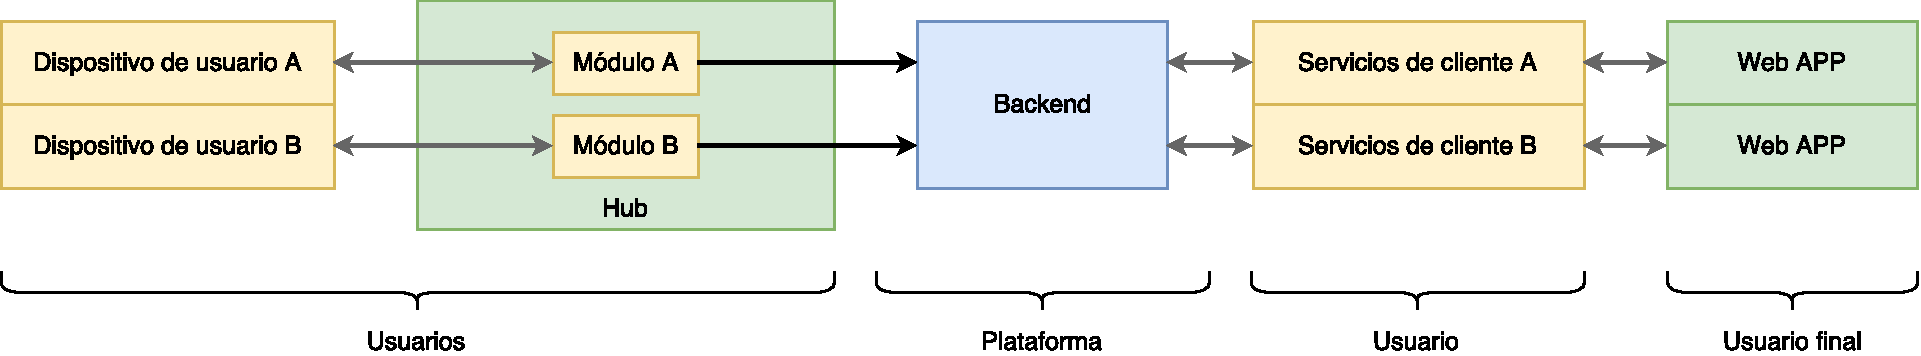
\includegraphics[width=\linewidth]{02-arquitectura/figuras/fig001}
\caption{Estructura de un aplicación que use la plataforma}
\label{fig:figura1}
\end{figure}

Como vemos en la \FIG{figura1}, la plataforma se sitúa como elemento intermedio entre
los dispositivos y la lógica del usuario. El objetivo es ofrecer de forma
transparente y eficiente un canal de comunicación al usuario para que éste pueda
centrarse en su negocio, que es ofrecer una serie de servicios al usuario final
sin tener que preocuparse por cómo se mueven los datos.

Puesto que la plataforma soporta multi tennant, múltiples usuario pueden
compartir la plataforma o una organización puede encargarse de mantenerla y
ofrecer sus servicios a los usuarios finales.

Sabiendo todo esto, podríamos definir la plataforma de la siguiente manera:

Es una plataforma que permite a los desarrolladores de dispositivos inteligentes
comunicar sus dispositivos con su lógica de negocio de forma transparente,
rápida, fiable y segura.
Para usar la plataforma habrá que preparar a los dispositivos que se distribuyan
para que se comuniquen con la API y por otro lado habrá que diseñar los
servicios para que obtengan los datos también de la API.

A continuación se puede ver un esquema de la arquitectura final en \FIG{figura2}.

\begin{figure}[htbp]
\centering
\includegraphics[width=\linewidth]{02-arquitectura/figuras/fig002}
\caption{Estructura interna de la plataforma}
\label{fig:figura2}
\end{figure}

\section{Componentes}

En la \FIG{figura2} se pueden ver los elementos de la plataforma, situados entre los
dispositivos y la lógica de negocio del usuario. Tenemos los siguientes
componentes:

\subsection{API}

Es el componente que permite a los usuarios comunicarse con la plataforma.
Tanto los dispositivos como los servicios propios del usuario usarán la API. Es
tarea de la API el registro de los dispositivos, el registro de usuarios y otras
tareas de gestión así como permite hacer consultas para obtener datos
almacenados en la plataforma.

La API es una aplicación que ha sido desarrollada como parte de este trabajo.
Se ha utilizado \texttt{Node.js} para su implementación.

\subsection{Broker}

Es el componente central de la arquitectura. Por él pasan
los mensajes enviados por los otros elementos. Permite balanceo de carga entre
múltiples instancias, persistencia, sincronización, etc.

Como \emph{broker} se ha usado \textbf{RabbitMQ} ya que es uno de los más
extendidos por su capacidad para escalar, su robustez y su extensibilidad.

\subsection{Bases de datos}

La persistencia del sistema. Múltiples bases de datos se
encargan de almacenar los datos recibidos que deben ser persistidos. También
será necesaria almacenar información de usarios y dispositivos registrados.

Para almacenamiento de credenciales se usará una base de datos \texttt{MongoDB}
por ser una de las más populares. Para persitir los datos del usuario que llegan
al sistema se usa \texttt{RethinkDB}. La característica más importante de esta
base de datos es que, a diferencia de las bases de datos convencionales, las
aplicaciones no tienen que consultarla de forma periódica para detectar nuevos
datos o modificaciones en éstos, sino que es la propia base de datos la que
notifica a las aplicaciones.

\subsection{Backend de autorización}

Debido a que es necesario controlar el acceso a la plataforma a los dispositivos
y a las aplicaciones, necesitamos un control de acceso. En este escenario, el control
de acceso debe realizarlo el \emph{broker}, en este caso en particular lo hará
\texttt{RabbitMQ}. Gracias a un plugin para éste, podemos delegar la autenticación
en una aplicación externa, de forma que el \emph{broker} realizará una petición
\texttt{HTPP} a una aplicación cuando un cliente se intente conectar, siendo esta
aplicación quien decida si se permite o no.

El \emph{backend de autorización} es la aplicacion encargada de tomar las decisiones.
Tendrá conectividad con la base de datos donde se encuentran las credenciales y
verificará que las conexiones son legítimas.

Esta aplicación también ha sido desarrollada como parte del trabajo, una vez más
usando \texttt{Node.js} como plataforma.

\subsection{Procesador de flujos}

Este componente obtiene los datos en crudo de la cola de
mensajes, los trata y los almacena en la base de datos. Puede ser interesante
añadir algunos metadatos a la información recibida antes de almacenarse.

Al mismo tiempo, la base de datos notificará a este componente cuando termine de
persistir el dato y este componente lo enviará a una cola del \emph{broker} donde
posteriormente podrá leerlo una aplicación que se conecte a la plataforma.

También se ha desarrollado como parte del trabajo en \texttt{Node.js}.

% !TEX root =../LibroTipoETSI.tex
\chapter{Node.js y arquitectura de microservicios}\LABCHAP{NODEJS}
\pagestyle{esitscCD}

% !TEX root =../LibroTipoETSI.tex
\chapter{Protocolo MQTT y STOMP}\LABCHAP{MQTT}
\pagestyle{esitscCD}

\section{MQTT}

\texttt{MQTT} es un protocolo cliente/servidor que permite roles de publicador/suscriptor.
Es ligero, abierto, simple y diseñado para ser fácil de implementar en el cliente.
Estas características lo hacen ideal para su uso en múltiples situaciones, como por ejemplo,
entornos donde la memoria y el ancho de banda son limitados, como la comunicación M2M
(\emph{Machine to machine}) o para dispositivos en el Internet de las Cosas.

Es un protocolo binario ligero que, en comparación con \texttt{HTTP}, tiene una
mínima sobrecarga en cuanto a cabeceras para hacer más eficiente el tampaño de los
paquetes.
\texttt{MQTT} es muy fácil de implementar en el cliente. Esto encaja perfectamente
en sistemas integrados con recursos limitados, de hecho,
esto es uno de los objetivos que se buscaban cuando \texttt{MQTT} se creó.

\subsection{El patrón publicador/suscriptor}

\begin{figure}[htbp]
\centering

\includegraphics[width=\linewidth]{04-mqtt/figuras/fig001}
\caption{Patrón publicador/suscriptor}
\label{fig:figura1}
\end{figure}

El patrón publicador/suscriptor es una alternativa al sistema tradicional de
cliente/servidor, donde un cliente se comunica directamente con un destino.
Sin embargo, el patrón \texttt{pub/sub} desacopla al cliente que están enviando
un mensaje (publicador) de otro cliente o más clientes que reciben mensajes
(suscriptor). Esto quiere decir que publicador y suscriptor no son conscientes
de la existencia del otro. Existe un tercer componente llamado \emph{broker} que
es conocido tanto por el publicador como el suscriptor que es el encargado de
filtrar los mensajes que llegan y distribuirlos correctamente.

As already mentioned the main aspect in pub/sub is the decoupling of publisher and receiver, which can be differentiated in more dimensions:
Como ya hemos mencionado, el pricipal aspecto del patrón publicador/suscriptor
es el desacople en las siguientes dimensiones:

\begin{itemize}\itemsep1pt \parskip0pt \parsep0pt
\item Espacio desacoplado: Publicador y suscriptor no tiene porqué saber el uno del otro (IP, puerto, etc.).
\item Tiempo desacoplado: Publicador y suscriptor no tienen porqué estar en ejecución al mismo tiempo.
\item Sincronización desacoplada: Las operaciones de los dos componentes no se detienen durante envío o recepción.
\end{itemize}

En resumen, el patrón publicador/suscriptor desacopla el publicador o receptor de
un mensaje y a través de los filtros para los mensajes se puede elegir qué clientes
reciben qué mensajes.

\subsection{Escalabilidad}

El patrón publicador/suscriptor ofrece mejor escalabilidad que el patrón clásico
de cliente/servidor. Esto se debe a que las operaciones en el broker pueden ser
altamente paralelizadas. También es común el cacheo de mensajes y el enrutado
inteligente. Sin embargo, es un reto el escalar a millones de conexiones, esto
puede conseguirse mediante el uso de clústeres de \emph{brokers} para distribuir
la carga entre múltiples servidores.

\subsection{Filtrado de mensajes}

El filtrado de mensajes es el encargado de que sólamente los mensajes sean
recibidos por los clientes que deben. Tenemos varias opciones de filtrado de
mensajes:

\begin{itemize}\itemsep1pt \parskip0pt \parsep0pt
\item Filtrado basado en \texttt{topic}: El \texttt{topic} puede ser parte de cada mensaje. Cada
cliente recibe sólamente mensajes del \texttt{topic} en el que está interesado. Los topics
generalmente son cadenas de texto organizadas de forma jerárquica, por lo que se puede
filtrar en función de una expresión.
\item Filtrado basado en contenido: El filtrado se basa en el contenido específico
del mensaje. Una gran desventaja de este método es que el contenido del mensaje
debe ser conocido por el \emph{broker}, cosa que no siempre ocurre, por ejemplo,
cuando el contenido va cifrado.
\item Filtrado por tipo: En lenguajes orientados a objetos es típico filtrar en
base a un tipo o clase del mensaje o evento. En este caso el suscriptor podría
recibir todos los mensajes de un tipo o subtipo.
\end{itemize}

En el caso de \texttt{MQTT} se utiliza el filtrado por \texttt{topic} así que cada
mensaje contiene un \texttt{topic}, el cual es procesado por el \texttt{broker}
para entregarlo a los clientes que se han suscrito a él.

\texttt{MQTT} tiene múltiples niveles de calidad de servicio (QoS). Se puede
conseguir fácilmente que un mensaje sea entregado del cliente al \emph{broker} o
del \emph{broker} al cliente. Sin embargo, existe la posibilidad de que nadie
se suscriba a un \texttt{topic} en particular, en este caso depende el \emph{broker}
cómo se debe manejar la situación.

\subsection{Diferencias con un sitema de colas}

Existe confusión debido a su nombre en cuanto a sí es un protocolo de colas.
Su nombre proviene de \emph{MQseries}, un producto de \emph{IBM} y no de \emph{Message Queue}.
Independientemente del nombre, existen diferencias entre \texttt{MQTT} y un
sistema de colas:

\begin{itemize}\itemsep1pt \parskip0pt \parsep0pt
\item Un sistema de colas almacena un mensaje hasta que se consume: En un sistema
clásico los mensajes se almacenan hasta que son tomados por un cliente (consumidor),
esto en \texttt{MQTT} no ocurre ya que puede haber cero clientes suscritos a un
topic y el mensaje es descartado.
\item Un mensaje sólo es consumido por un cliente: Otra gran diferencia es el hecho
de que en un sistema tradicional de cola de mensajes, los mensajes son consumidos
por un único consumidor así la carga se puede distribuir entre múltiples procesos.
En \texttt{MQTT} esto suele ser al contrario, todos los suscriptores reciben el
mensaje si se han suscrito al \texttt{topic}.
\item Las colas tienen nombres y deben crearse de forma explícita: Una cola es
menos flexible que un \emph{topic}, antes de usar una cola debe declarase
explícitamente y sólo entonces se pueden consumir los mensajes. En \texttt{MQTT}
los \emph{topics} son extremadamente flexibles y son creados en el momento.
\end{itemize}

% !TEX root =../LibroTipoETSI.tex
\chapter{Protocolo AMQP y RabbitMQ}\LABCHAP{AMQP}
\pagestyle{esitscCD}

AMQP (Advanced Message Queuing Protocol) es un protocolo de mensages que permite
a aplicaciones de clientes comunicarse con un broker.

\section{Brokers}

Los brokers de mensajes reciben los mensajes de los publicadores (aplicaciones
que los publican, también conocidos como productores) y los enrutan hacia los
consumidores (aplicaciones que los procesan).

Ya que es un protocolo de red, los publicadores, consumidores y el broker pueden
residir en diferentes máquinas.

\section{El modelo AQMP}

El modelo de AMQP 0-9-1 tiene la siguiente visón de lo que ocurre:

Los mensajes se publican en \emph{exchanges}, que se podrían ver como un buzón
o una oficina postal. Los \emph{exchanges}, al recibir mensajes, los distribuyen
a las colas (\emph{queues}) siguiendo unas reglas llamadas \texttt{bindings}.
A continuación, el \emph{broker} entrega los mensajes a los consumidores
que están suscritos a las colas, o los propios consumidores consultan la cola
y leen los mensajes.

\begin{figure}[htbp]
\centering
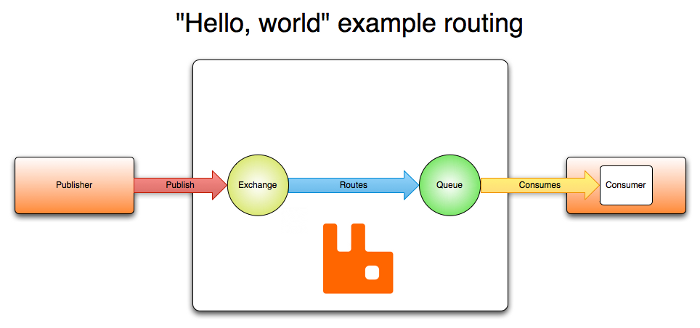
\includegraphics[width=\linewidth]{05-amqp/figuras/fig001}
\caption{Ejemplo de enrutamiento en AMQP}
\label{fig:figura1}
\end{figure}

Cuando se publica un mensaje, se pueden especificar diferentes atributos (\emph{metadata}).
Alguno de estos atributos pueden ser usados por el \emph{broker}, sin embargo,
el cuerpo del mensajes es completamente opaco para el \emph{broker} y sólamente
será usado por la aplicación que recibirá el mensaje.

Las redes pueden tener problemas y las aplicaciones puede fallas al procesar los
mensajes, por eso mismo, el modelo \texttt{AMQP} hace uso de \texttt{ACKs}. Cuando
un mensaje se entrega a un consumidor, éste debe notificar al broker que ha procesado
el mensaje, ya sea de forma automática o cuando el desarrollador de la aplicación
lo decida. El \emph{broker} sólamente eliminará el mensaje de la cola cuando
éste haya sido confirmado.

En algunas situaciones, por ejemplo, cuando un mensaje no puede ser enrutado,
el mensaje puede ser devuelto al productor, descartado o, si el broker lo implementa,
enviado a una cola especial llamada \emph{dead letter queue}. Los consumidores pueden
elegir cómo manejar situaciones como estas usando algunos parámetros a la hora de
publicar los mensajes.

Las colas, los \emph{exchanges} y los \emph{bindings} son conocidas como
\textbf{entidades de AMQP}-

\section{\emph{Exchanges}}

Los \emph{exchanges} son entidades de AMQP a donde llegan los mensajes. Éstos
al recibir los mensajes los enrutan hacia cero o más colas. El algoritmo de
enrutado depende del tipo de \emph{exchange} y las reglas definidas (\emph{bindings}).
Existen cuatro tipos de \emph{exchanges}:

\begin{itemize}\itemsep1pt \parskip0pt \parsep0pt
\item Direct exchange: \texttt{amq.direct}
\item Fanout exchange: \texttt{amq.fanout}
\item Topic exchange:	\texttt{amq.topic}
\item Headers exchange:	\texttt{amq.match}
\end{itemize}

Independientemente del tipo de \emph{exchange}, éstos son declarados con ciertos
atributos, los más importantes son:

\begin{itemize}\itemsep1pt \parskip0pt \parsep0pt
\item Name: Nombre del \emph{exchange}.
\item Durability: Indica al \emph{broker} que debe sobrevivir a
reinicios.
\item Auto-delete: Son eliminados sin no hay ninguna cola asociada.
\item Arguments: Dependen del \emph{broker}.
\end{itemize}

\subsection{\emph{Direct Exchange}}

Los \emph{exchanges} directos entregan los mensajes a las colas basándose en
la \texttt{routing key}. Son ideales para enrutamiento \emph{unicast}, aunque
también se pueden usar para \emph{multicast}. Funcionan de la siguiente manera:

\begin{itemize}\itemsep1pt \parskip0pt \parsep0pt
\item Una cola se conecta (establece un \emph{binding}) al \emph{exchange} con
la \texttt{routing key} \texttt{K = R}
\item El \emph{exchange} directo suele ser usado para distribuir mensajes entre
múltiples \emph{workers} en modo \emph{round robin}. Es importante ser conciente
de que en \texttt{AMQP} se balancea entre consumidores y no entre colas.
\end{itemize}

Se puede ver de forma grágica en la \FIG{figura2}.

\begin{figure}[htbp]
\centering
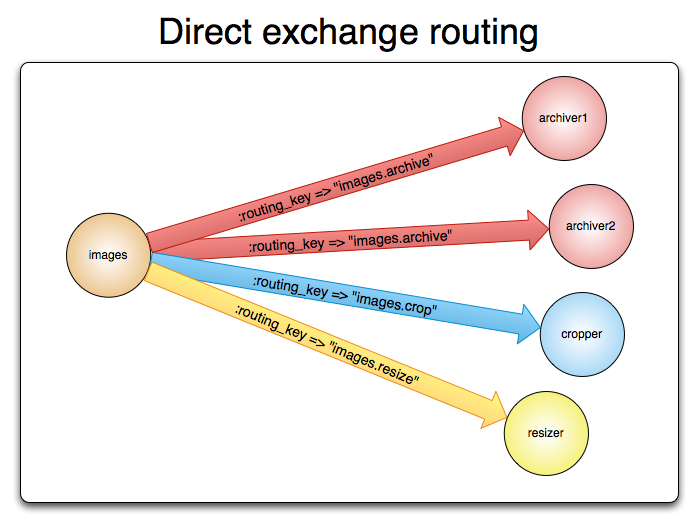
\includegraphics[width=0.75\linewidth]{05-amqp/figuras/fig002}
\caption{\emph{Exchange} directo}
\label{fig:figura2}
\end{figure}

\subsection{\emph{Fanout Exchange}}

Este tipo de \emph{exchange} enruta todos los mensajes a todas las colas con las
que está conectado, es decir, la \texttt{routing key} se ignora en este caso.
Una copia de cada mensaje es enviado a cada una de las colas. Este tipo de
\emph{exchange} es ideal para el tráfico \emph{broadcast}.

Se puede ver de forma grágica en la \FIG{figura3}.

\begin{figure}[htbp]
\centering
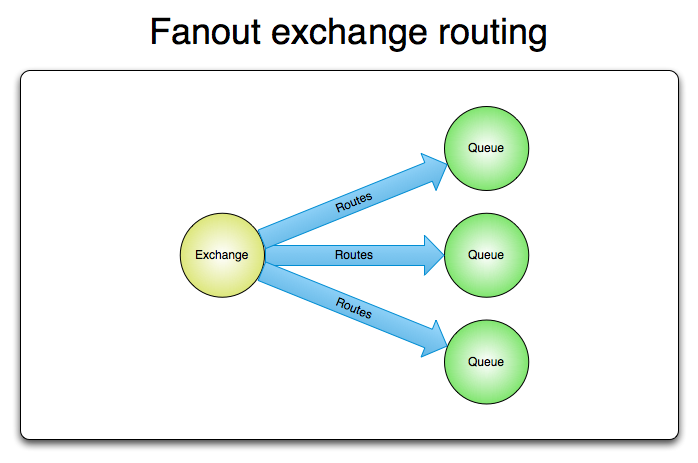
\includegraphics[width=0.75\linewidth]{05-amqp/figuras/fig003}
\caption{\emph{Fanout exchange}}
\label{fig:figura3}
\end{figure}

\subsection{\emph{Topic Exchange}}

En este caso, los mensajes se envían a una o varias colas, basándose en la
\texttt{routing key} con la que una cola está conectada a un \emph{exchange}. Este
patrón se suele usar en modelos de publicador/suscriptor.

\subsection{\emph{Header Exchange}}

El \emph{header echange} está diseñado para enrutar mensajes basándose en múltiples
atributos que viajan en las cabeceras de los mensajes en lugar de usar la
\texttt{routing key}.

\section{Colas}

Las colas en \texttt{AMQP} son muy similares a las colas en otros sistemas de
colas. Almacenan mensajes que pueden se consumidos por aplicaciones. Las colas
comparten algunas propiedades con los \emph{exchanges}, pero también tienen sus
propios atributos:

\begin{itemize}\itemsep1pt \parskip0pt \parsep0pt
\item Name: Nombre de la cola.
\item Durable: Indica al \emph{broker} que deben sobrevivir a
reinicios.
\item Exclusive: Sólo se permite una conexión a la cola.
\item Arguments: Dependen del \emph{broker}.
\end{itemize}

Las colas deben ser declaradas antes de poder ser usadas. La declaración hace que
la cola se cree si no existía anteriormente, si ya estuviese declarada, otra
declaración no tendrá ningún efecto. Si se vuelve a declarar con otros atributos
diferentes, se producirá una excepción.

\subsection{Colas durables}

Las colas durables se persisten a disco y sobreviven a reinicios del \emph{broker},
en cambio, las colas que no son durables son llamadas transitorias. No todos los
escenarios requieren que una cola sea durable.

La durabilidad de una cola no hace que los mensajes que sean enrutados hacia esa
cola sean durables. Si el \emph{broker} se reinicia, las colas durables volverán
a declararse durante el inicio de forma automática, sin embargo, sólamente los
mensajes persistidos podrán recuperarse.

\section{\emph{Bindings}}

Los \emph{bindings} son reglas usadas por los \emph{exchanges} para enrutar los
mensajes recibidos hacia las colas. Para que un \emph{exchange} enrute un mensaje
a una cola, dicha cola debe enlazarse con el \emph{exchange}. Los \emph{bindings}
pueden tener atributos opcionales como las \texttt{routing keys}. La finalidad
de una clave de enrutado es seleccionar ciertos mensajes publicados en un \emph{exchage}
que está enlazado con una cola, es decir, actúan como filtros.

Cuando un mensaje no se puede enrutar hacia una cola se descartará o se devolverá
al productor, dependiendo de los atributos que el productor haya ajustado.

\section{Mensages}

Los mensajes en \texttt{AMQP} tienen atributos. Algunos de ellos son tan común
que la especificación los define de forma que los desarrolladores no tienen que
preocuparse por ellos.

\begin{itemize}\itemsep1pt \parskip0pt \parsep0pt
\item Content type
\item Content encoding
\item Routing key
\item Delivery mode
\item Message priority
\item Message publishing timestamp
\item Expiration period
\item Publisher application id
\end{itemize}

Algunos atributos los usa el \emph{broker}, pero la mayoría de ellos son para
los consumidores que lo reciben. Algunos atributos
son opcionales. Los atributos se fijan cuando el mensaje se publica.

Los mensajes también tienen una carga (los datos) que el \emph{broker} trata
como una ristra de \emph{bytes}. El \emph{broker} no inspecciona o modifica
los datos. Es bastante común enviar los datos serializados en formatos como
\texttt{JSON}, \texttt{MessagePack}, \texttt{Protocol BUffers}, etc. Para comunicar
esta información se pueden usar los atributos \texttt{content-type} o \texttt{content-encoding}.

Los mensajes pueden ser publicados como persistentes, que hace que el \emph{broker}
los persista a disco. Si el servidor se reinicia, el sistema se asegura que los
mensajes persistentes no se pierdan. Sólo por publicar un mensaje en un \emph{exchange}
durable o que la cola a la que el mensaje es enrutado sea durable no hace que el
mensaje sea persitido, para ello el mensaje tiene que ser publicado como persistente.
Hay que tener en cuenta que publicar mensajes persistentes afecta al rendimiento.

\chapter{Dispositivos y Módulos}\LABCHAP{DISPS}
\pagestyle{esitscCD}

\section{Dispositivos}

Los dispositivos son elementos externos al sistema. El propio sistema está
diseñado para proveer servicios a estos dispositivos, por lo que podemos verlos
como un especie de usuario de la plataforma.

Cada dispositivo debe estar registrado en el sistema para poder interactuar con
él, por lo que deberán implementar un proceso en el cual puedan darse de alta en
la plataforma. Cada dispositivo estará asociado a un usuario, esto quiere decir
que a la hora de registrarse, el dispositivo debe proveer cierta información
para que la plataforma pueda determinar a qué usuario quedará asociado.

\subsection{Flotas}

La forma de asociar un dispositivo a un usuario es mediante las \textbf{flotas}.
Las flotas son agrupaciones independientes de dispositivos que puede crear el
usuario para gestionarlos. Cada usuario puede tener múltiples flotas. Al crear
una flota, se generará de forma automática una \texttt{fleet\_key}, que es una clave única
que representa a cada flota. Cuando un dispositivo ejecuta el proceso de
registro deberá proveer la clave para que el sistema lo reconozca como
perteneciente a su flota correspondiente a la hora de registrarlo en la base
de datos.

Dispositivos de diferentes flotas no pueden comunicarse entre ellos de forma
directa, es decir, si en una flota un dispositivo publica en el \emph{topic}
\texttt{temperature} y otro dispositivo de una flota diferente está suscrito
a este \emph{topic} no recibirá el mensaje. Sin embargo, siempre será posible
que una aplicación o dispositivo pertenezca a ambas flotas y sea capaz de
reenviar los mensajes.


\section{Módulos}

Los módulos son aplicaciones que simulan ser dispositivos. Su objetivo es actuar
como intermerdiario entre los dispositivos reales y la plataforma.

El dispositivo en el que corren los módulos se denominará hub. Una Raspberry Pi
puede ser muy adecuado como hub ya que puede implementar los protocolos
necesarios y puede comunicarse con los dispostivos reales usando un adaptador
Bluetooth o ZigBee.

Existen varios escenarios donde puede ser interesante usar módulos:

\subsection{Caso 1}
Los dispositivos no tienen capacidad de enviar mensajes \texttt{HTTP} o \texttt{MQTT}, que son los
protocolos usados por la plataforma. En tal caso, se puede crear un módulo que
corra en otro dispositivo capaz de implementar estos protocolos y, al mismo
tiempo, sea capaz de comunicarse con los dispositivos reales. Estos módulos
tienen la responsabilidad de registrarse como si fuesen dispositivos reales,
obtener datos y reenviarlos a los dispositivos correspondientes. Útiles para
dispositivos que usan \texttt{Bluetooth} o \texttt{ZigBee} como protocolo de comunicación.

\subsection{Caso 2}
Los dispositivos ya existen y no es posible modificar el software para que se
comunique con la plataforma directamente. Por ejemplo porque los dispositivos
los fabrica un tercero. En este caso, el módulo tiene una función de ``pasarela''
entre los dispositivos reales y la plataforma.

\section{Conexión al broker}

Para enviar datos a la plataforma será necesario disponer de los siguientes datos:

\begin{itemize}\itemsep1pt \parskip0pt \parsep0pt
\item \texttt{host}: El nombre o dirección IP del equipo donde está desplegada la plataforma.
\item \texttt{puerto}: El puerto donde se reciben los mensajes de los dispositivos mediante \texttt{MQTT}.
\item \texttt{user}: El \texttt{uuid} del dispositivo, generado en el proceso de registro.
\item \texttt{password}: La contraseña del dispositivo, generada en el proceso de registro.
\item \texttt{topics}: \texttt{<fleet\_key>/\#}. Donde ``\#'' es el nombre original del topic.
\end{itemize}

A la hora de publicar mensajes en un topic, el dispositivo debe preceder el
topic con el \texttt{fleet\_key}, por ejemplo, si se quiere publicar al topic
``temperature'', deberá enviarse el mensaje al topic \texttt{<fleet\_key>/temperature}.

Para suscribirse a un topic se aplicará la misma regla, precediendo el nombre
del topic original por el Fleet Key.

Se debe usar usar TLS ya que sino las credenciales viajarán en texto plano y
pueden ser capturadas por un tercero.

\chapter{API}\LABCHAP{API}
\pagestyle{esitscCD}

Lo primero y más importanta del sistema son los usuarios. Serán quienes exploten
las funcionalidades del sistema. Puesto que la finalidad de la plataforma es
establecer una comunicación entre los dispositivos de un cliente y su lógica,
tenemos dos roles:

\begin{itemize}\itemsep1pt \parskip0pt \parsep0pt
\item \indexit{Dispositivos:} Los componentes que obtienen información o
controlan elementos.
\item \indexit{Lógica:} El software del usuario que procesan la información
obtenida y controlan los dispositivos.
\end{itemize}

Para que el usuario pueda interactuar con la plataforma para conocer el estado
de los dispositivos se proveerá de una API RESTful que permita:

\begin{itemize}\itemsep1pt \parskip0pt \parsep0pt
\item \indexit{Registro de usuarios}
\item \indexit{Administración de flotas}
\item \indexit{Monitorización de dispositivos}
\end{itemize}

\section{Registro de usuario}

Para crear un usuario se enviará un mensaje HTTP a la API con el contenido del
código \ref{pet-01}:

\begin{minipage}{\textwidth}
\begin{lstlisting}[language=TeX,caption={Petición para creación de usuario}, breaklines=true, label=pet-01]
POST /users

{
  "email": "yo@dominio.com",
  "password": "secreto"
}
\end{lstlisting}
\end{minipage}

Una vez registrados, se puede hacer login y realizar peticiones autenticadas a
la API. Para realizar un \emph{login} debemos enviar el contenido del código \ref{pet-01}.

\begin{minipage}{\textwidth}
\begin{lstlisting}[language=TeX,caption={Petición de login}, breaklines=true, label=pet-02]
POST /users/login

{
  "email": "yo@dominio.com",
  "password": "secreto"
}
\end{lstlisting}
\end{minipage}

Como respuesta se obtiene el \texttt{acess\_token} y \texttt{user\_id}:

\begin{minipage}{\textwidth}
\begin{lstlisting}[language=TeX,caption={Respuesta a login}, breaklines=true, label=res-01]
{
  "id": "<access_token>",
  "ttl": 1209600,
  "created": "2013-12-20T21:10:20.377Z",
  "userId": "<user_id>"
}
\end{lstlisting}
\end{minipage}

A partir de ahora podemos realizar peticiones autorizadas enviando en la
cabezera del mensaje \texttt{HTTP} el \texttt{access\_token} el campo
  \texttt{Authorization}.

\section{Obtención de Fleet Key}

Para crear una flota es necesario haber realizado el proceso de registro y
disponer de un \texttt{user\_id} y \texttt{acess\_token}. Ser realizará la
petición indicada en el código \ref{pet-03}.

\begin{minipage}{\textwidth}
\begin{lstlisting}[language=TeX,caption={Creación de \texttt{fleet\_key}}, breaklines=true, label=pet-03]
POST /users/<user_id>/fleets

Authorization: <access_token>
\end{lstlisting}
\end{minipage}

Si todo ha ido correctamente se obtendrá como respuesta el mensaje de respuesta
\ref{res-02}

\begin{minipage}{\textwidth}
\begin{lstlisting}[language=TeX,caption={Obtencion de \texttt{fleet\_key}}, breaklines=true, label=res-02]
{
  "uuid": "<fleet_uuid>"
}
\end{lstlisting}
\end{minipage}

\section{Registro de dispositivos}

Cuando el dispositivo se inicie por primera vez, deberá realizar un proceso de
registro en el que usará la \texttt{fleet\_key} para poder obtener un
\texttt{uuid} y un \texttt{secret}. Para que un dispositivo pueda registrarse deberá ser capaz de comunicarse
mediante \texttt{HTTP}, en caso contrario, será necesario el uso de un dispostivo
intermedio capaz de realizar esta labor en nombre del dispositivo.

A este dispositivo intermedio lo llamaremos \texttt{hub} que puede ser cualquier
dispositivo que sea capaz de enviar mensajes \texttt{HTTP} y \texttt{MQTT} y
reenviarlos en el protocolo que sea a los dispositivos reales. Podría ser, por
ejemplo, un \emph{router} o una \emph{Raspberry Pi}.

Un caso podría ser un \emph{Arduino} que se comunicase mediante un módulo \texttt{NRF24} con
un programa que se ejecute en una \emph{Raspberry Pi}. Será dicho programa de la
\emph{Raspberry Pi} el responsable de realizar el registro, de forma que el dispositivo no
tiene porqué tener conocimiento del proceso ni de la plataforma. Cabe destacar
que, en este caso, será la aplicación en cuestión quien debe conocer la \texttt{fleet\_key}.

Esto puede ser útil en caso de tener dispositivos que no podemos adaptar al
sistema, bastaría con crear este intermediario para poder usar el dispositivo
con la plataforma.

En cualquier caso, el procedimiento será enviar un mensaje \texttt{HTTP} a la
API con el contenido de la petición \ref{pet-04}.

\begin{minipage}{\textwidth}
\begin{lstlisting}[language=TeX,caption={Registro de dispositivo}, breaklines=true, label=pet-04]
POST /fleets/<fleety_key>/registerMote
\end{lstlisting}
\end{minipage}

\begin{minipage}{\textwidth}
\begin{lstlisting}[language=TeX,caption={Respuesta de registro de dispositivo}, breaklines=true, label=res-03]
{
  "uuid":   "<Nuevo UUID de dispositivo>",
  "secret": "<Nuevo secreto>"
}
\end{lstlisting}
\end{minipage}

Una vez obtenidas las credenciales para poder enviar datos deberían persistirse
para futuros usos.


%%:Empezamos con los apéndices, que irían en uno o más ficheros.
%% Es necesario incluir estos ficheros entre el entorno
%% \begin{appendices}....\end{appendices} debido a que se ha deseado utilizar
%% un formato diferente para el título de los apéndices, incluyendo la palabra
%% apéndice, para la numeración de los apéndices, alfabético, y para las
%% cabeceras de las páginas.
% \begin{appendices}
% \include{apendices/apendices} %Ver este fichero para incluir ahí los apéndices.
% \end{appendices}

\backmatter

%:Indice de figuras, coméntese las siguientes líneas si no se desea
\cleardoublepage
\phantomsection

%:Para añadir una línea en blanco en el TOC y separar esta lista
\addtocontents{toc}{\protect\mbox{}\protect\hspace*{0pt}\par}
\addcontentsline{toc}{listasb}{\listfigurename}
\pagestyle{especial}
\listoffigures

%:Indice de Programas
\cleardoublepage
\phantomsection
\addcontentsline{toc}{listasb}{\lstlistlistingname}
\pagestyle{especial}
\lstlistoflistings

%:Bibliografía con biblatex y biber
\cleardoublepage
\phantomsection
\addcontentsline{toc}{listasb}{\bibname}
\pagestyle{especial}
%BIBER
%\printbibliography[heading=etsi]
%BIBTEX
%\bibliographystyle{IEEEtran}
\bibliographystyle{amsplain} %flexbib amsplain alpha
%:Fichero con la bibliografía, BIBTEX
\bibliography{bibliografiaLibroETSI}

\end{document}
